%%%%%%%%%%%%%%%%%%%%%%%%%%%%%%
% Manipulation 
%%%%%%%%%%%%%%%%%%%%%%%%%%%%%%
\subsection{Manipulation}\label{sec:manipulation}
As mentioned before, I tested a linear (\textit{InterFaceGAN)} and a non-linear (\textit{StyleFlow}) approach, both from the family of supervised latent space manipulation techniques. Due to its low editing performance and prohibitively high computational cost, \textit{StyleFlow} has been disregarded after initial editing experiments on physical attributes like color or sleeve length of a dress. \textit{InterFaceGAN} on the other hand was used throughout all experiments in this work.

\subsubsection{InterFaceGAN}\label{sec:interfacegan}
The latent space of StyleGAN models is smoothly interpolable \citep[p.1]{stylegan1} and gradual changes in one direction in the latent space of a well-trained generator can result in gradual changes in a specific semantic attribute \citep[p.6]{bermano2022state}. \cite{shen2020interpreting} propose a simple, yet effective method of finding this direction in a method called \textit{InterFaceGAN}. The method is based on the assumption that for any binary semantic, a hyperplane in the latent space can be found that separates the two classes \citep[p.3]{shen2020interpreting}. Assuming a hyperplane with a unit normal vector $\mathbf{n} \in \mathbb{R}^d$, with $d$ being the dimension of the latent space, the "distance" of the latent representation of sample $\mathbf{z}$ to the hyperplane can be defined as 
\[d(\mathbf{n, z}) = \mathbf{n}^T\mathbf{z}.\]
If one moves towards and across the hyperplane in the latent space, the sign of the distance changes, and thus the semantic attribute in the generated image should have changed to the opposite class \citep[p.3]{shen2020interpreting}. 

\begin{wrapfigure}{r}{6cm}
    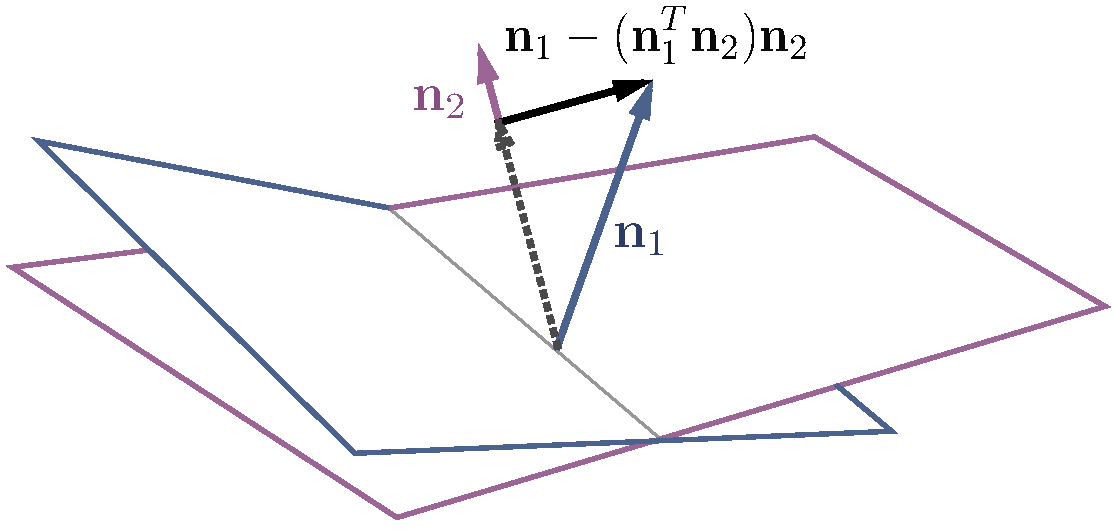
\includegraphics[width=6cm]{Thesis/Method/assets/subspace_projection.pdf}
    \caption[Conditional manipulation via subspace projection]{Conditional manipulation via subspace projection - taken from \cite{shen2020interpreting}, p.4}
    \label{fig:subspace_projection}
\end{wrapfigure} 

While this is straightforward for a single binary attribute, often multiple semantics are present and might not be independent of each other, although the latent space of StyleGAN models already enforces some degree of disentanglement (see section \ref{sec:gans}). In the case of $m$ semantics, $m$ separation boundaries $\mathbf{N} = [\mathbf{n_1, ..., n_m}]$ can be found. To disentangle them, $\{\mathbf{n_1, ..., n_m}\}$ need to be orthogonal to each other \citep[p.4]{shen2020interpreting}. In practice, conditional manipulation, i.e. editing one semantic without affecting any other semantic, can be performed using projection. As illustrated in figure \ref{fig:subspace_projection}, if one wants to manipulate the semantic connected with the hyperplane $\mathbf{n_1}$ without affecting the semantic connected with $\mathbf{n_2}$, the projection of  $\mathbf{n_1}$ onto $\mathbf{n_2}$ is subtracted from $\mathbf{n_1}$. Thus, the conditional manipulation direction is
$$\mathbf{n_{cond}} = \mathbf{n_1} - (\mathbf{n_1}^T\mathbf{n_2})\mathbf{n_2}.$$
For the semantic editing, the authors apply a simple linear manipulation of the latent space in the positive or negative direction of the unit normal vector $\mathbf{n}$ of the separation boundary. Thus the manipulated latent representation is defined as
$$\mathbf{z}_{edit} = \mathbf{z} + \alpha\mathbf{n},$$
with the synthesis being more positive on the semantic for $\alpha >0$ and more negative with $\alpha <0$ \citep[p.4]{shen2020interpreting}.

Since \textit{InterFaceGAN} is a supervised approach, either labels for the semantics or classifier scores need to be available. If there are labels available, those can directly be used to find a hyperplane that separates the latent space based on these labels. If only classifier scores are available, the authors propose to use the samples with the highest and lowest scores and assign binary labels. The hyperplane is then found by training a simple linear classifier on the latent representations. In this case, a linear Support Vector Machine (SVM) is trained. Linear SVMs learn a decision boundary which acts as the separation boundary in latent space that is used by InterFaceGAN.

\subsubsection{Training}\label{sec:interfacegan_training}

To make the \textit{InterFaceGAN} approach usable for this work, some implementation details needed to be adapted. While the authors used the 512-dimensional $\mathcal{Z}$-space of StyleGAN, I used the 16x512-dimensional $\mathcal{W^+}$-space. Thus, finding a hyperplane in this higher dimensional space is not as straightforward as in $\mathcal{Z}$. To tackle this problem, one could either flatten the latent representation in $\mathcal{W^+}$-space by concatenating all 16 dimensions along one dimension or learn 16 separate hyperplanes, one for each of the dimensions. The latter results in individual manipulations in each of the 16 dimensions. As explained in section \ref{sec:gans}, the various dimensions of $\mathcal{W}$ and $\mathcal{W^+}$ are injected at different levels of the synthesis process and allow targeted variations at different scopes of the image. Thus, learning isolated separation boundaries allows to apply targeted manipulation in the specific semantic only at a certain coarseness level of the generation process. On the other hand, learning one separation boundary from the complete latent representation allows the linear classifier to consider all features at all levels at the same time when finding the manipulation direction. Both approaches have been implemented and tested and the results are very similar. Since the isolated boundaries approach requires another step of selecting the dimensions to consider in the manipulation, the method of flattening the latent space has been selected as the final approach, thus simplifying the process without sacrificing editing performance. \\
When constructing the training data for the typicality scores, I closely follow the authors of \textit{InterFaceGAN} by using only the top $n$ and bottom $n$ scores in the classifier training. The idea is to create two distinct classes that can be clearly separated and that exhibit strong attributes of the two classes, i.e. high and low typicality. The boundaries have been computed using values of $n=1000$, $n=2000$, and $n=3000$. Finally, the separation accuracy on a separate validation set has been computed and the boundary with the best accuracy was selected as the final manipulation direction. \\
Another difference in the \textit{InterFaceGAN} implementation between this work and the original approach is the nature of the semantics. While the authors could show that the approach works well on naturally binary attributes like gender or the presence of glasses in facial images, or ordinal features like the age of a person, the labels present in the dresses dataset are different. Physical attributes like color or sleeve length, which are used as conditioning factors in the typicality manipulation, are nominal and have high cardinality. For those attributes, $\frac{n!}{2!(n-2)!}$ hyperplanes are calculated with $n$ being the number of unique values an attribute has. Therefore, there are hyperplanes for each combination of binary directions in the feature space. Defining one attribute value as positive while assigning all the others to the negative class (one-vs-rest) leads to multiple problems. First of all, the linear classification problem becomes extremely imbalanced. Furthermore, according to \cite{yang2021discovering} that set of negative samples provides ambiguous or even misleading guidance to the linear classifier, resulting in entangled semantics and incorrect manipulation directions \citep[p.1]{yang2021discovering}. When choosing a specific boundary as the conditional boundary, the set of boundaries to choose from is restricted to those that cover the real attribute value. So if the conditioning is on the color attribute and the dress is blue, all boundaries that include "blue" together with any other color are candidates. Out of the candidates, the boundary that has the best accuracy on the validation set during the classifier training is chosen. To visually validate the quality of these physical attribute boundaries, some preliminary manipulation tests using physical attributes have been run. The results of these experiments can be found in the appendix in figure \ref{fig:physical_attributes_manipulation}. Furthermore, descriptive statistics for the multiple separation performances of the physical attributes can be found in table \ref{tab:physical_summary_stats} in the appendix.



